\section{Measurements Results}

Initially, the operating levels of each of the evaluated receptors were collected, presented in the table ref{tab: receivers}, through the determination of the reception threshold as described in the previous section. These measures were used as a reference for comparing the results of the. 

% Tabela receptores
%=========================================================
\begin{table}[h!]
	\begin{center}
		\centering
		\caption{ISDB-T Receivers operational level}
		\label{tab:Receptores}
		\begin{tabular}{|l|c|c|c|c|}
			\hline
			\textbf{Receptor} & \textbf{RX1} & \textbf{RX2} & \textbf{RX3} & \textbf{RX4}\\
			\hline
			Power Level (dBm/6MHz)&-75,7 & -75,2 & -79,7 & -75,1\\
			\hline
			Power Level (dBm/18MHz)&-75,2 & -73,7 & -77,9 & -73,8\\
			\hline
		\end{tabular}
	\end{center}
\end{table}
%=========================================================

%Limiar de saturação (Oth) para interferência de canal adjacente
\begin{table*}[t!]
	\begin{center}
		\centering
		\caption{ $O_{th}$ para teste de interferência em canais adjacentes}
		\label{tab:Resultados_ADJ01}
		\begin{tabular}{|c|c|c|c|c|c|c|c|c|}
			\hline
			\textbf{Receptores}&\multicolumn{2}{c|}{\textbf{RX1}}&\multicolumn{2}{c|}{\textbf{RX2}}&\multicolumn{2}{c|}{\textbf{RX3}}&\multicolumn{2}{c|}{\textbf{RX4}}\\
			\hline
			\textbf{Canal UHF}&\textbf{31}&\textbf{33}&\textbf{31}&\textbf{33}&\textbf{31}&\textbf{33}&\textbf{31}&\textbf{33}\\
			\hline
			\textbf{OFDM (dBm/6MHz)} &-53,4&-53,1&-54,4&-53,6&-53,2&-53,6&-53,6&-53,4\\
			\hline
			\textbf{GFDM (dBm/6MHz)} &-47,3&-47,4&-50,1&-50,2&-49,3&-49,2&-49,2&-49,3\\
			\hline
			\textbf{W-GFDM (dBm/6MHz)}&-38,0&-39,8&-41,2&-41,2&-42,8&-39,7&-41,2&-41,1\\
			\hline
			\textbf{F-OFDM (dBm/6MHz)}&-38,5&-38,6&-41,7&-40,3&-43,5&-39,7&-41,2&-40,2\\
			\hline
		\end{tabular}
	\end{center}
\end{table*}
%=========================================================

\begin{figure}[h]
    \centering
    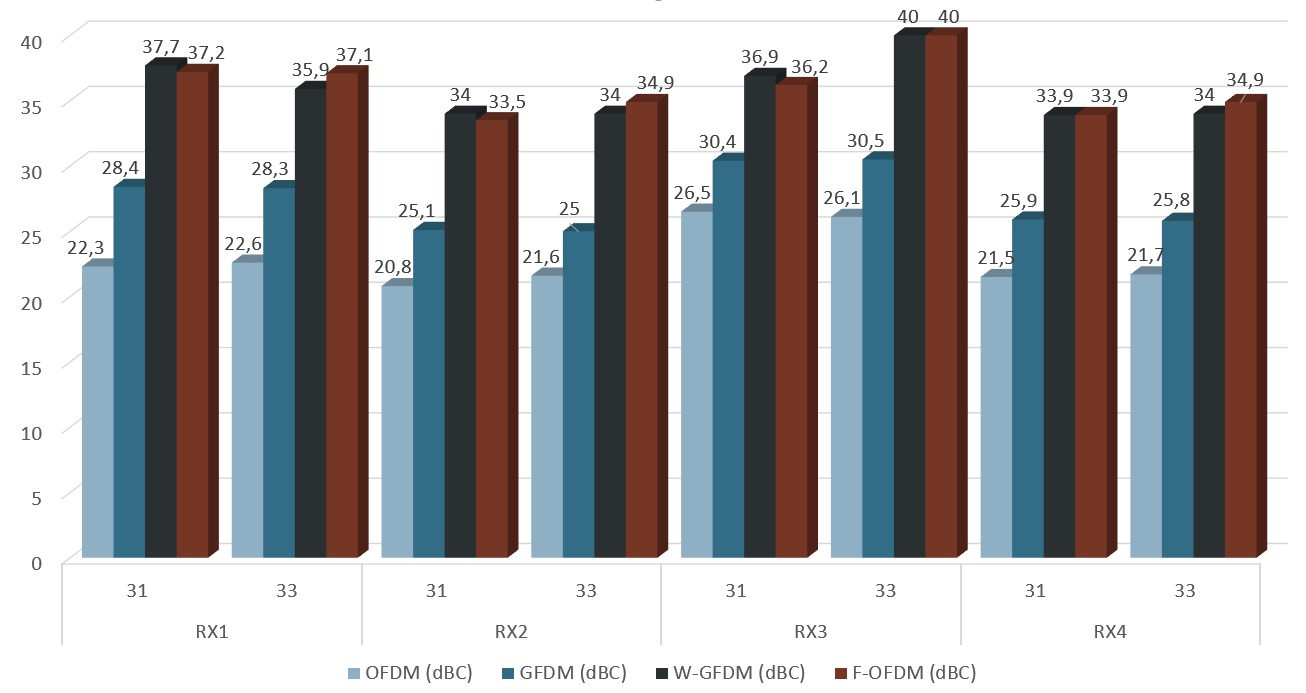
\includegraphics[width=0.48\textwidth]{Figures/result_01.jpg}
    \caption{$O_{th}$ Comparrisson with ISDB-T operational level for adjacent channel test (dBc)}
    \label{fig:result_01}
\end{figure}

%=========================================================

%Limiar de saturação (Oth) para interferência com sinal ocupando multiplos canais
\begin{table}[h!]
	\begin{center}
		\centering
		\caption{$O_{th}$ medido em ensaio de interferência com sinais ocupando múltiplos canais}
		\label{tab:Resultados_ADJ02}
		\begin{tabular}{|c|c|c|c|c|}
			\hline
		    \textbf{}&\textbf{RX1} & \textbf{RX2} & \textbf{RX3} & \textbf{RX4}\\
			\hline
			OFDM (dBm/18MHz) &-65,25&-65,2&-68,2&-66,8\\
			\hline
			GFDM (dBm/18MHz) &-59,2&-60,7&-63,7&-63,0\\ 
			\hline
			W-GFDM (dBm/18MHz) &-42,2&-41,9&-43,9&-43,2\\
			\hline
			F-OFDM (dBm/18MHz) &-65,3 &-65,2&-68,3&-66,9\\
			\hline
		\end{tabular}
	\end{center}
\end{table}

%=========================================================

\begin{figure}[h]
    \centering
    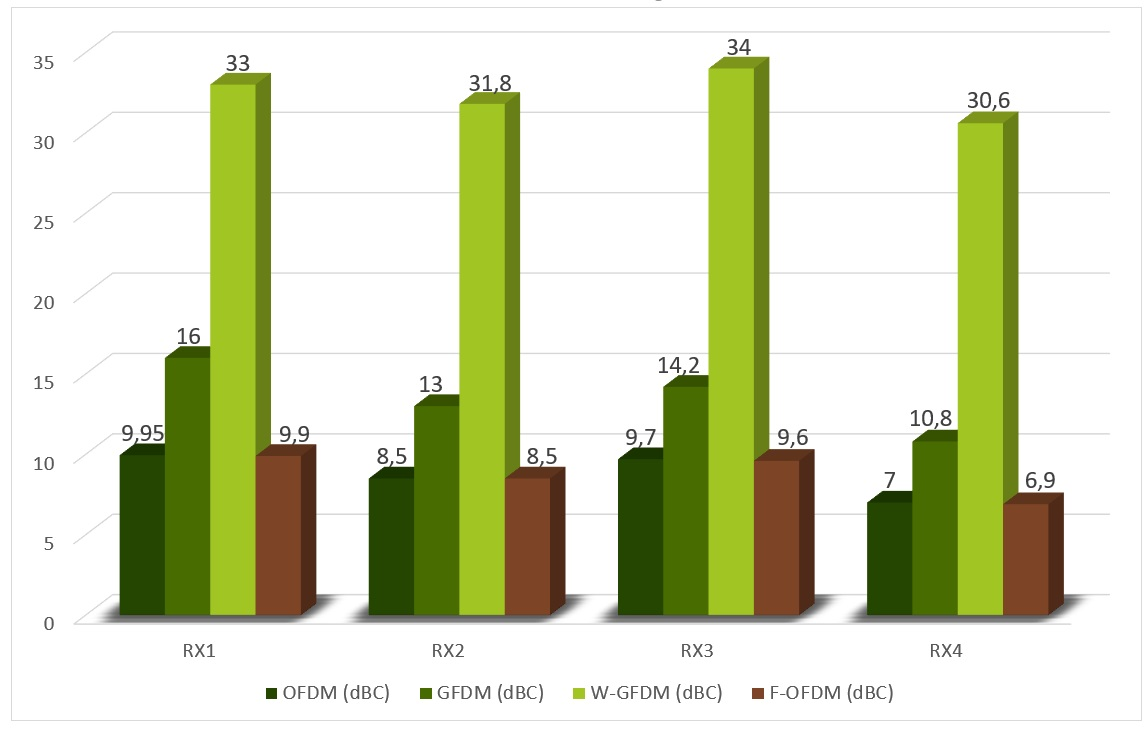
\includegraphics[width=0.48\textwidth]{Figures/result_02.jpg}
    \caption{$O_{th}$ Comparrisson with ISDB-T Operational Level for multiple channel test (dBc)}
    \label{fig:result_02}
\end{figure}

%=========================================================

Comparing the measurements of $O _{th} $ shown in the table ref{tab: Resultados_ADJ01} for the interference test on adjacent channels it is verified that the F-OFDM and W-GFDM transmission techniques caused harmful interference operating at the level of Higher power in all tested equipment. Making the relationship with the operating threshold, as shown in Figure ~ ref{fig: result_01} It is noted that in this experiment there was no significant difference between these technologies. par

%=========================================================

In the experiment with signals operating in multiple channels and disconnected carriers, as shown in table ref{tab: Resultados_ADJ02}, once again it was found that the W-GFDM transmission technique interfered with the primary service, with the highest level. In this scenario the $O _th $ for the modulated signal in F-OFDM practically showed no advantages when compared to OFDM, as can be seen in Figure ~ ref{fig: result_02}. We believe that this result is due to the type of prototype filter used in base-band signal generation and deeper studies should be done to mitigate this problem. par
%=========================================================

The results of the measurements indicated that out-of-band emissions for the modulations proposed for 5G are lower when compared to the OFDM technique. Figure ~ ref{fig: Waveforms} illustrates this situation, where you can see the difference between the technologies by measuring the spectral densities of power. The more efficient use of the PC gives the W-GFDM greater spectral efficiency and energy savings when compared to the other modulations analyzed. This feature is important in the WRAN scenario, where the major delays of channel paths require long cyclical prefixes cite{IEEE_802_22}. Therefore, this is quite promising for operations in texti{white spaces}. par
%=========================================================

\begin{figure}[h]
    \centering
    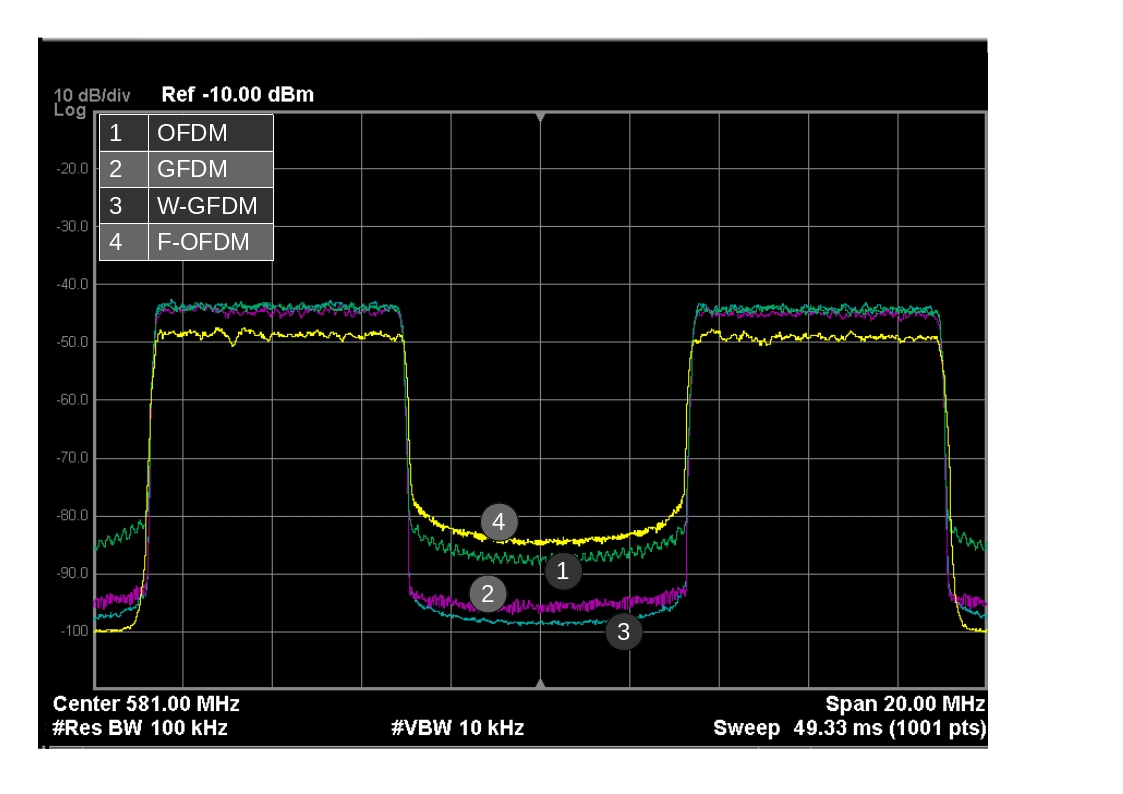
\includegraphics[width=0.48\textwidth]{Figures/5G_WaveformsCompare.jpg}
    \caption{Waveforms out of band emission comparision}
    \label{fig:waveforms}
\end{figure}